% !TeX root = ../document.tex

\section{Discussion}

In this study only local and small areas with occurring heat islands where detected. The \ldq{}heat islands effect\rdq{} was not set into context with the surrounding areas of Berlin, because we intended to focus on the intra-urban heat islands effect only. Moreover, our decision was based on a lack of data outside the metropolitan area. Within the urban area the stations were evenly distributed as shown in figure \ref{fig:station_dsitribution} and are thus suitable for several of the interpolation methods. It should be emphasized that the stations are subject to different microclimates and as such are influenced by parks, large sealed areas or open water. \cite{chowienczyk_estimating_2020} Also, technical failure of the measuring instruments are possible and need to be taken into account. These effects were not studied in detail, but could have a significant impact on the results. Because detailed analysis of the stations, their location and immediate surroundings was not possible, the pre-processing of the raw data was an important step in order to receive more accurate and reliable data without outliers. Some of these outliers could be identified and omitted in the further process. However, the reliability and accuracy of the data depends on the choice of method for detecting and removing the outliers, which leaves some uncertainty and needs further evaluation. 

Overall, openSenseMap is definitely a good starting point for a first analysis of the regional characteristics. It provides relevant data and one can even explore data online by using the provided interpolation tool. However, the data needs to be treated with caution and a thorough review is recommended. Generating more precise results could be achieved by comparing the data to official values such as data from the DWD (Deutscher Wetterdienst).  
In terms of validation, we’d suggest contrasting both datasets. Another approach would be to leave out random stations, then carry out the interpolation and afterwards examine if the omitted stations fit with the interpolated data. This would of course only expedient, if sufficient and adequat data is available. 
As stated before, the choice of different interpolation methods was made by sighting of literature and studies with similar approaches or a relevant thematic focus. The results of the identified methods show how different certain areas are depicted. Certainly a further analysis of methods and also FOSSIGIS tools could lead to more scientifically valid statements, but none of the methods does guarantee that the results will be accurate if the research question and the data that has to be evaluated does not “fit” with the choice of method. 
While Nearest neighbor and TIN have proven to be rather unsuitable for identifying specific heat islands within a city, IDW and Spline provided a more detailed and differentiated outcome. It remains to be examined in how far the created connections between single “islands” (especially in regard to Spline interpolation - compare figure 9) are plausible and which factors contribute to the generated local rise in temperature. The advantage with Spline is that is predicts values lying outside the of the sample point dataset, however, abrupt temperature variations and large differences between the single points are smoothed out and were not preserved. But these sudden temperature changes and shifts are imaginable, especially if vegetated areas border artificial, dark or other heat accumulating surfaces that can heat up easily when exposed to direct sunlight. 
The comparison of the IDW methods carried out with GDAL and GRASS GIS has opened up some new questions. Although the parameters (max neighbors and power factor) were identical, the results show slightly – and towards the outer edges rather large – differences. While the “heat islands” detected through GDAL (compare figure 8(a)) show a more north-south expense, with some of the islands connecting, the results obtained from the calculations through GRASS GIS offer a different picture. Here the “heat islands” seem to be stretched east-west (compare figure 8(b). In this regard, further investigations could unfold why these distinctive discrepancies occurred. 

% TODO: Fix citation above
% TODO: Focus on answering: choice of data, aggregation and quality of data/ choice of method and parameters (power factor)/ discuss the results and differences 

% TODO: How can this resaerch be applied to other areas?
% TODO: How can be optimized?
% TODO: Which questions araise after the analysis?
% TODO: Outlook: compare differen options (power factor, etc.) for suitability

\begin{figure}[H]
	\centering
	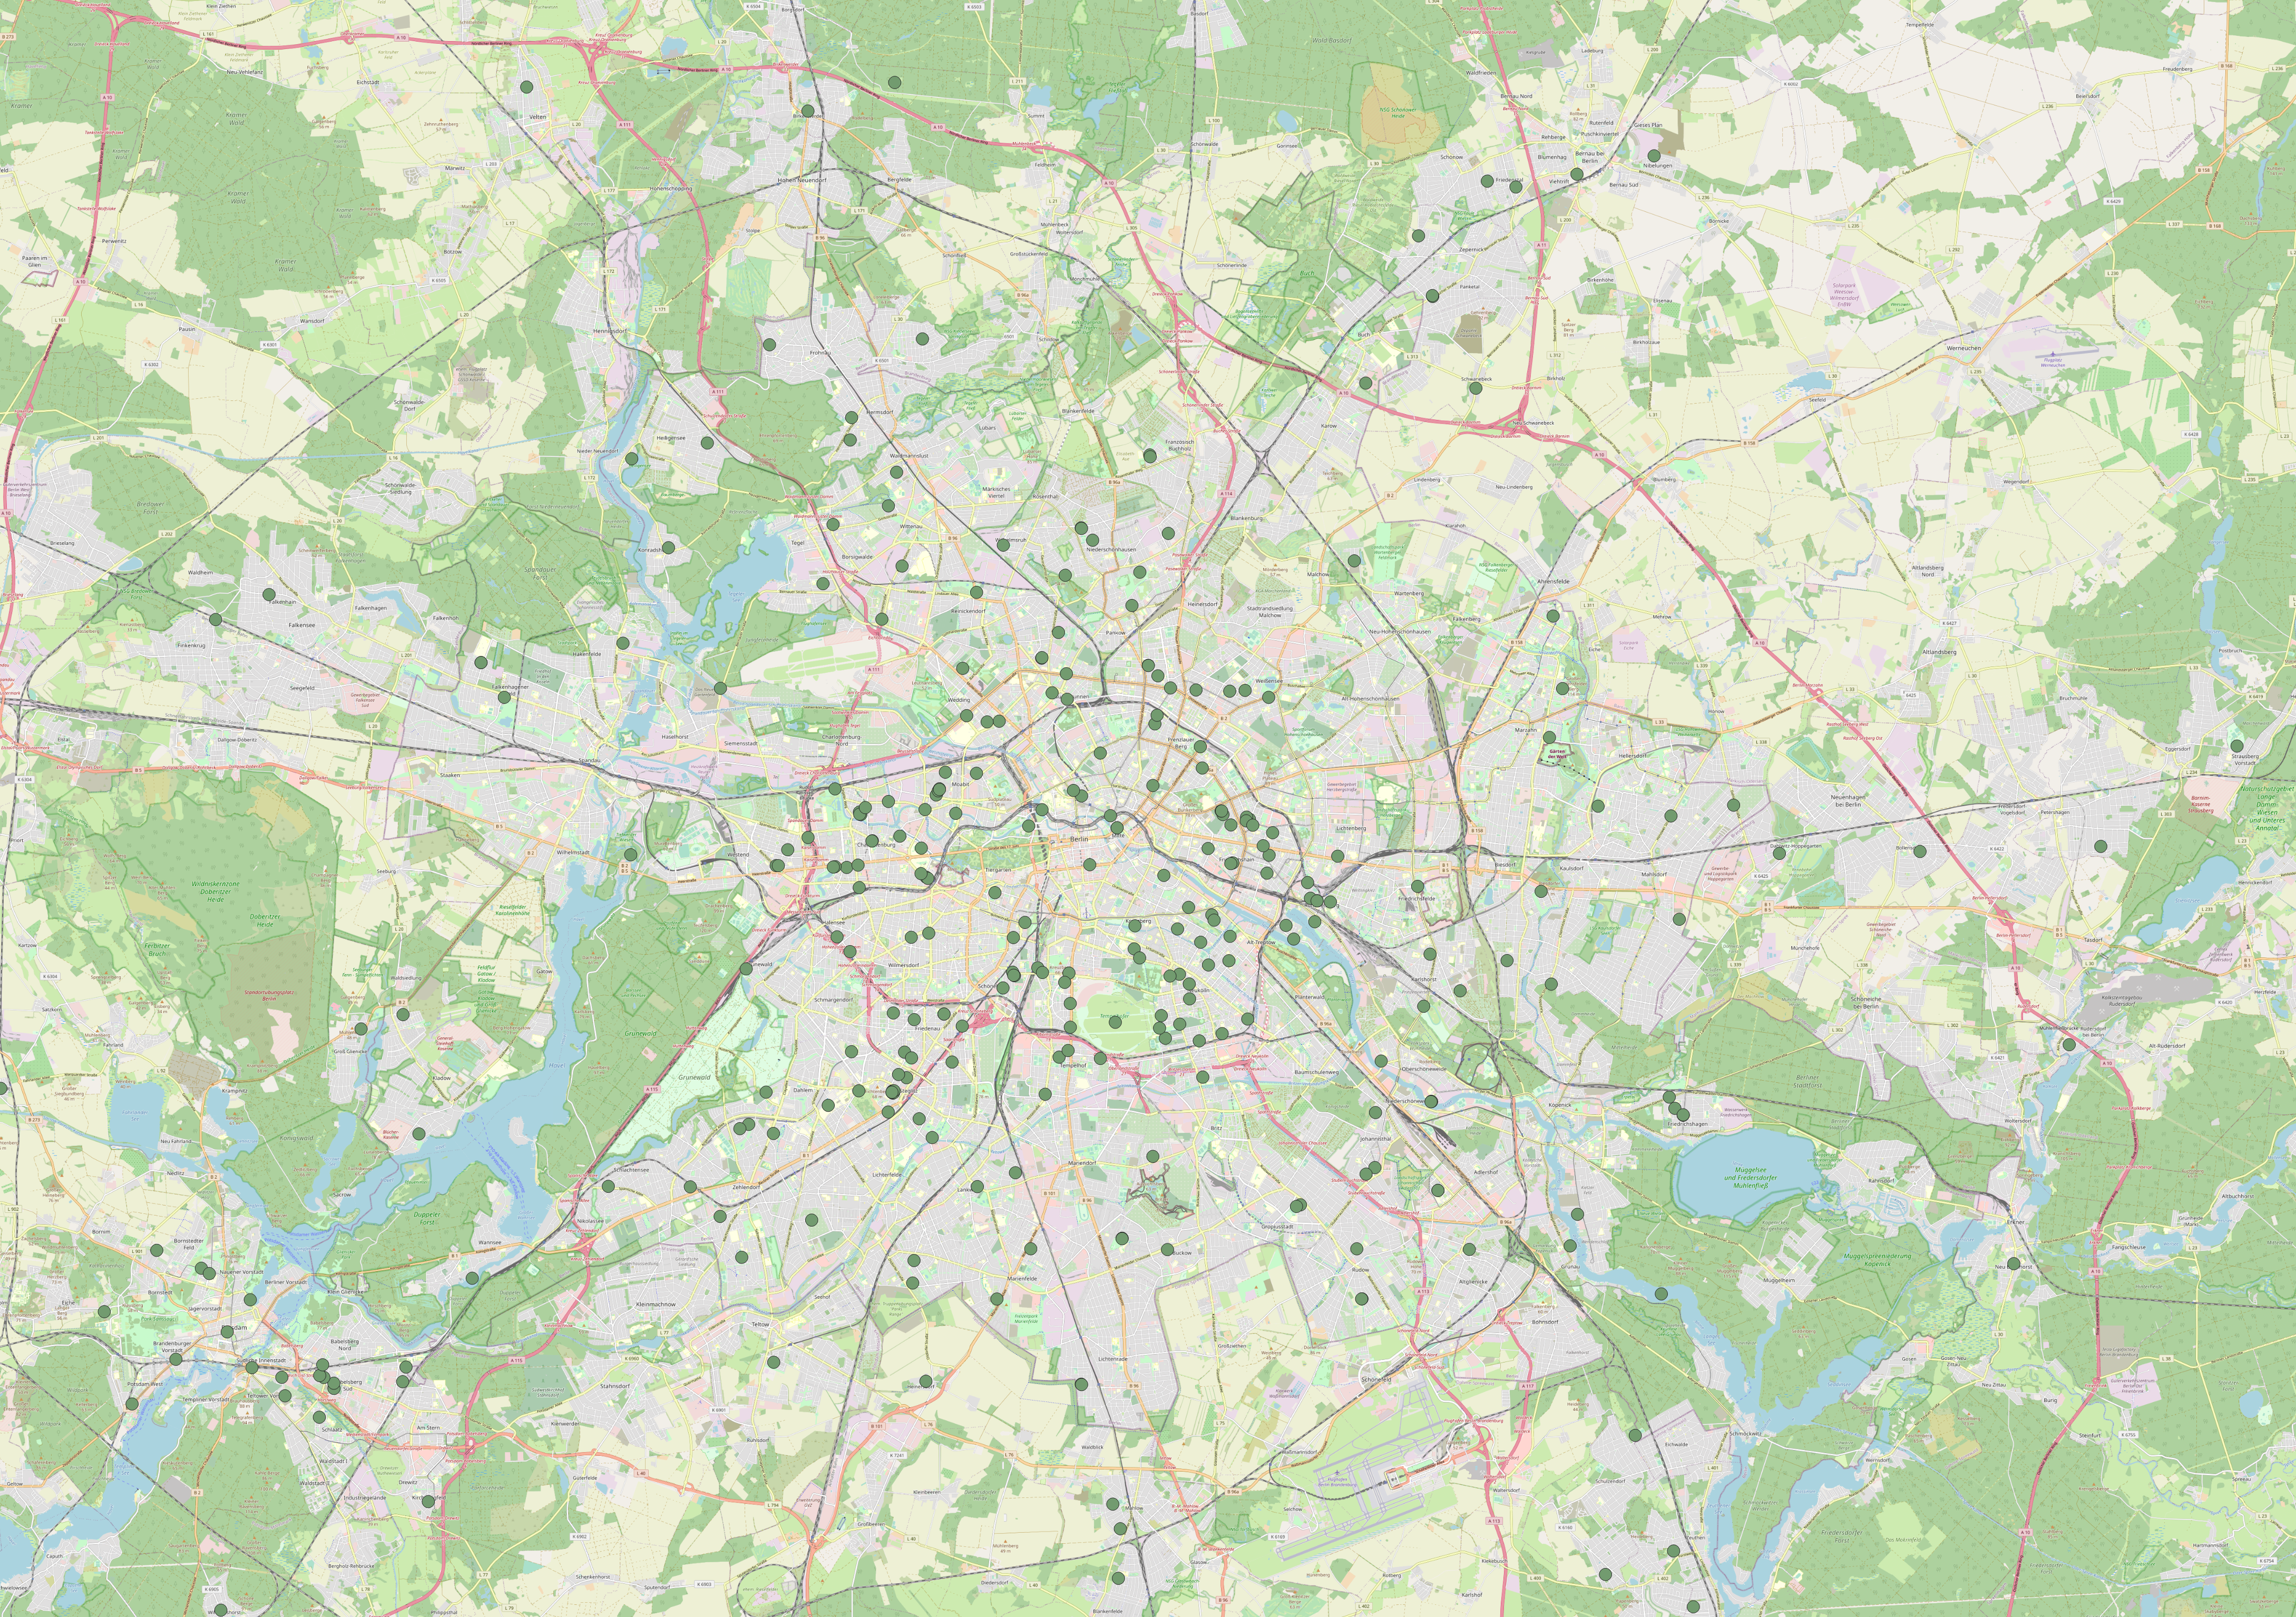
\includegraphics[width=.7\linewidth]{images/station_distribution.png}
	\caption{Distribution of sensor stations that measure the \ldq{}Temperatur\rdq{} phenomenon}
	\label{fig:station_dsitribution}
\end{figure}
